
\subsection{Color-correction for point-sources of various spectral indices}
\label{ap:color_correction_JFL}

Adopting  the ``NIKA2 photometric system'' convention, the response of a NIKA2 detector in Analog-to-Digital Unit and over the bandpass 
of transmission $T_{\nu}$ to Uranus is :

$$ R_{ADU}^{ura} =  S_{\nu_0}^{ura}~ k~\int_{0}^{+\infty} (\nu /\nu_0)^{1.6} ~ T_{\nu} ~ d\nu  $$

\null

\noindent or : $$ R_{ADU}^{ura} = K_{ura}  ~ S_{\nu_0}^{ura} $$

\null

\noindent The conversion factor   $K_{ura}  = k ~
\int_{0}^{+\infty} (\nu /\nu_0)^{1.6} ~ T_{\nu} ~ d\nu $ can be
determined with a beam-map on Uranus in taking the ratio between the measurement $R_{ADU}^{ura}$ of each detector and 
the adopted flux density of Uranus $S_{\nu_0}^{ura}$ at the reference frequency $\nu_0$ (150 or 260 GHz).
Note that the SED of Uranus taken here as $\propto (\nu)^{1.6}$  is undistinguishable of a more
accurate atmospheric model  (Moreno/ESA) for our purpose.


For a target of spectral indice  $\alpha_{S}$ that is different from Uranus,  
its  response in Analog-to-Digital Unit $R_{ADU}^{sou}$    and over the bandpass
of transmission $T_{\nu}$ must be first converted to Jy/beam by means of the factor $K_{ura}$ :

$$ S_{\nu_0}^{~sou} =  {R_{ADU}^{~ sou} \over K_{ura}} $$

\noindent And then, a ``color-correction'' must be applied to account for the fact the SEDs of the target (likely $\alpha_{S} \ne 1.6$) 
and of Uranus ($\alpha=+1.6$) convolve differently with
each NIKA2 bandpass (Fig. \ref{fig:Trans}). The color-corrected flux density ${S'}_{\nu_0}^{~sou}$ can be expressed as :

$$ {S'}_{\nu_0}^{~sou} =  {R_{ADU}^{sou} \over { K_{ura} \times {{{\int_{0}^{+\infty} (\nu /\nu_0)^{\alpha_{S}} ~ T_{\nu} d\nu }  } \over { \int_{0}^{+\infty} (\nu /\nu_0)^{1.6} ~ T_{\nu} d\nu  }}}}  $$


\noindent where the proper conversion factor of the target source 
$K_{sou}=k ~ \int_{0}^{+\infty} (\nu /\nu_0)^{\alpha_S} ~ T_{\nu} d\nu $ substitutes factor $K_{ura}$.  Equivalently but more readily, the complete conversion formula is  :

$$  {S'}_{\nu_0}^{~sou} =  S_{\nu_0}^{~sou} \times {{ \int_{0}^{+\infty} (\nu /\nu_0)^{1.6} ~T_{\nu} d\nu   }  \over { \int_{0}^{+\infty} (\nu /\nu_0)^{\alpha_S} ~ T_{\nu} d\nu }   } $$

\null

\noindent with the color-correction factor ${{ \int_{0}^{+\infty} (\nu
    /\nu_0)^{1.6} ~T_{\nu} d\nu   }  \over { \int_{0}^{+\infty} (\nu
    /\nu_0)^{\alpha_S} ~ T_{\nu} d\nu }}$ computed  in the
Table below for 8 values of  $\alpha_{S}$, and in particular
for $\alpha_{S}= 0.6$ which is the spectral indice of MWC349.

\begin{table*}[!h]
\caption{Color correction factor correction for a target source  $S \propto \nu ^{\alpha_S}$}
\label{tab:mod}
\centering 
\begin{tabular}{l| c c c c c c c c}
\hline\hline
\noalign{\smallskip}
Array  & \multicolumn{8}{c}{$\alpha_{S}$} \\
\hline
          &  -2 &  -1    &    0  & + 0.6 & +1  &  +2  & +3 & +4  \\
%            \noalign{\smallskip}
            \hline
%            \noalign{\smallskip}
          A1   & 0.876  &  0.916   &   0.951  & 0.969 &  0.981   &  1.005  &    1.024  &  1.037   \\
          A2   & 0.945  &  0.972   &   0.990  & 0.996 &  0.998   &  0.997  &    0.986  &  0.966      \\ 
          A3   & 0.907  &  0.940   &   0.967  & 0.980 &  0.987   &  1.001  &    1.009  &  1.011     \\
            \noalign{\smallskip}
            \hline
\multicolumn{8}{c}{Note : Uranus/Moreno model used for Uranus in this Table.}
\end{tabular}
\end{table*}




\null
\null

\begin{figure}
    \centering
    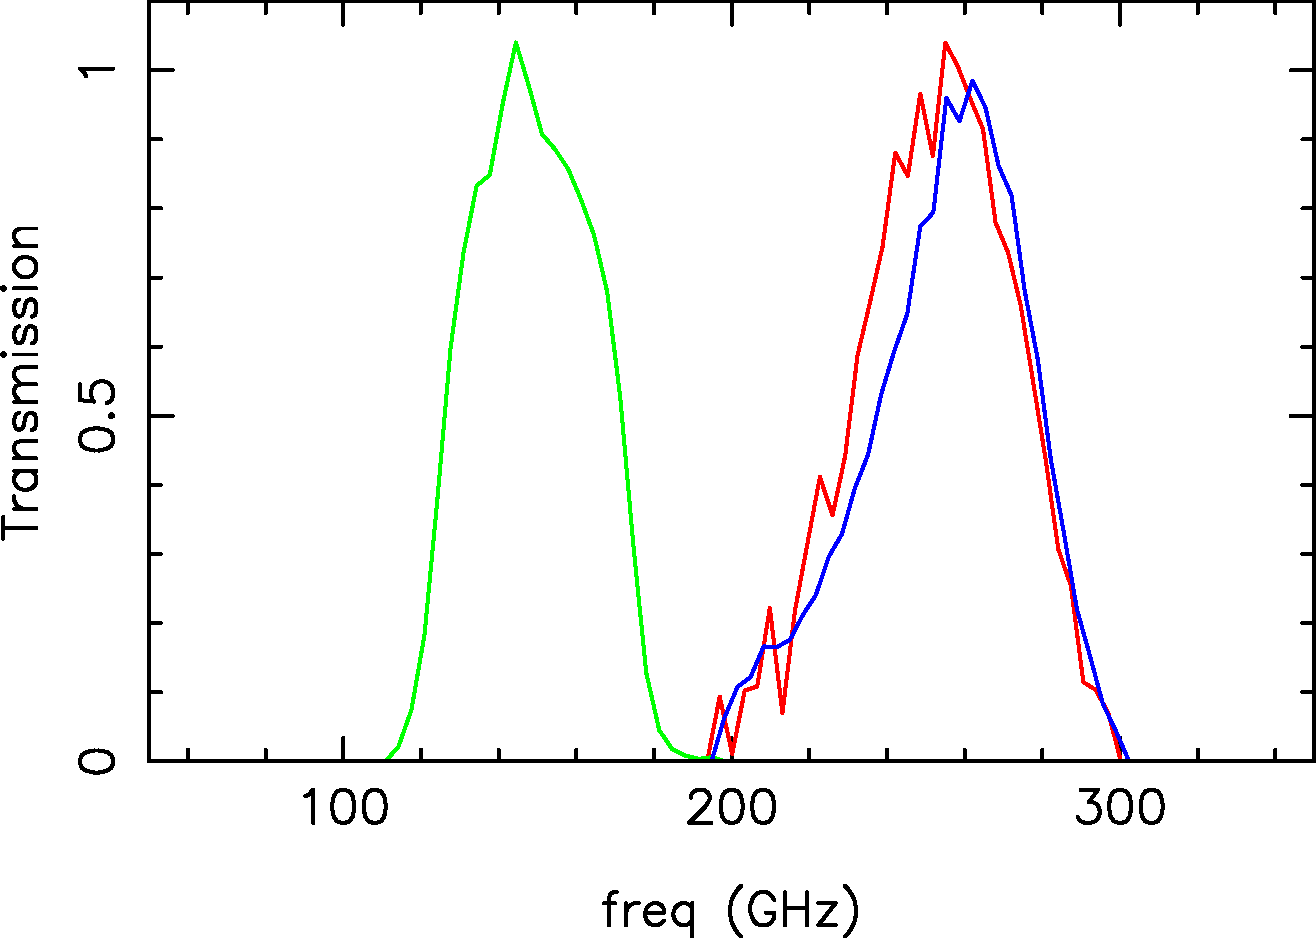
\includegraphics[width=0.60\textwidth]{Figures/Transmission-2017-Jan-NIKA2-v1.pdf}
    \caption{Transmissions $T_{\nu}$ for arrays A1, A2, A3 obtained
      from reponses to a black body (Transmission-2017-Jan-NIKA2-v1.fits) and then divided by
      $(\nu/\nu_0)^2$.} 
    \label{fig:Trans}
\end{figure}


